\chapter{Data sources}

This chapter presents the datasets used in the model estimation and validation. The first section provides details about the data sources and their main characteristics. The second section presents an exploratory data analysis that guides the prior definition and model specification in the next chapter. The final section focuses on the dataset's hierarchical structure, a key component of the model specification. 

Several datasets and surveys were evaluated before the model estimation. However, only the Survey of Labour and Income Dynamics (SLID) was considered suitable for developing the model. \Cref{table:datasource} presents all datasets reviewed for this work, and the following list explains the main reasons for using the SLID survey over the existing datasets. 

\begin{itemize}
    \item Cross-sectional labour market surveys such as the LFS are designed to provide a most representative view at the population level and to track general trends in the labour market. However, the longitudinal nature of SLID provides a more detailed view of the individuals and their dynamics within the labour market, such as transitions, durations, and occurrences of individual financials and work situations \citep{StatsCAN2012}.

    \item SLID provides more detailed information about the characteristics of the individuals, such as age, prior experience, education level, and other characteristics associated with the job. In contrast, LFS age and education level are grouped into fewer categories. LFS does not report previous work experience, which, according to the literature, is one of the most important predictors of a worker's salary. 
    
    \item Salary in SLID is reported annually, which provides a better estimate of the annual income from labour sources. Conversely, salaries in the LFS are reported as hourly wages, which can be difficult to calculate for many full-time workers. 
    
    \item Given that the LFS panel rotates every six months, and a panel is added every month, the salary estimates, and other representative variables can vary between periods. In contrast, the SLID panel is more stable and can produce more reliable estimates for the same variables. 
    
    \item Although the SLID dataset could be considered outdated when this thesis is written, labour market changes take longer. Therefore, this dataset still contains essential information about the dynamics of the labour market that can be applied today. One argument supporting its use is that the Industry and Occupation classification system has had only minor changes and additions at the subcategory level. However, the structure remains the same as the one used in the SLID survey\footnote{In 2022, Statistics Canada released a major change in the occupation classification system that organizes occupations in TIERS according to the education and skill level required for the job. However, these TIERS are just a subgroup of the original NOC categories used in this thesis.}. 
\end{itemize}

\renewcommand{\arraystretch}{1.5}
\begin{table}[H]
    \begin{tabular}{p{4cm}p{7cm}p{2.5cm}p{2.5cm}}
        \textbf{Dataset} & \textbf{Description} & \textbf{Frequency} & \textbf{Reference periods} \\
        \hline
        \rowcolor{lightgray} Labour Force Survey (LFS) & A cross-sectional survey that estimates the state of the labour market in Canada & Monthly & 1987-2022 \\
        
        Survey of Labour and Income Dynamics (SLID) & A longitudinal survey focused on understanding the labour market activity, household income, and the changes experienced by individuals and families through time & Annual & 1994-2011 (Discontinued) \\

        \rowcolor{lightgray} Survey of Older Workers (SOW) & A cross-sectional survey to identify the factors that influence the decision to retire or remain working. & One time & 2008 \\

        Canadian Income Survey (CIS) & A cross-sectional survey to monitor the income and sources of individuals and their household characteristics & Annual & 2012-2018 \\

        \rowcolor{lightgray} Employment and Insurance Coverage Survey (EICS) & Cross-sectional survey monitoring the Employment Insurance (EI) program. This survey provides an overview of the socio-economic characteristics of the unemployed and those not in the labour force. Also, it covers maternity and parental benefits. & Annual & 2007-2018 \\
        \hline
    \end{tabular}
    \caption{\label{table:datasource} Review of publicly available data sources related to the Labour Market}
\end{table}















\section{Survey of Labour and Income Dynamics - SLID }

The Survey of Labour and Income Dynamics (SLID) was a statistical program developed by Statistics Canada between 1993 and 2011 to investigate the Canadian population's income sources. This survey provides an additional perspective to the labour market surveys focused on the individual's characteristics. After 2011, this survey was discontinued, and some modules were included in the monthly Labour Force Survey. 

The SLID is a household longitudinal survey applied across all provinces and territories in Canada and collected by telephone. The sample, a subsample of the Labour Force Survey, consists of two panels of households of around 17,000 households and 34,000 respondents interviewed once a year for six years. A new panel was introduced every three years, so there was always an overlap of three years \citep{StatsCAN2012}. 

Although the original SLID is a longitudinal survey, the Public-Use Microdata File (PUMF) available on the Statistics Canada website corresponds to the cross-sectional version of the survey. That means all identifiers that track individuals within the panel are not provided. Statistics Canada applies this transformation to preserve data privacy and confidentiality. Similarly, geographic information is aggregated at the province level. Given that the wage model proposed in this thesis is part of the ILUTE model, the SLID dataset is filtered to include samples from Ontario to match the geographical context of the ILUTE model. 

SLID dataset consists of a set of 147 variables in its last version (2011). These variables are grouped into the following five categories that represent some characteristics of the individual, their household, or their labour status at the time of the survey. According to the theoretical foundations discussed in the literature review, these variables are filtered to select the most relevant for modelling salaries. \Cref{table:model_vars} details the variables used for the model specification. 

\renewcommand{\arraystretch}{1.5}
\begin{table}[H]
    \begin{tabular}{p{2.5cm}p{5.5cm}p{7cm}}
        \textbf{Variable group} & \textbf{Variable subgroups} & \textbf{Variables used in the model} \\
        \hline
        \rowcolor{lightgray} Sample & Identifiers, Sample variables & Personal identifier, Survey year, Sample weight. \\

        Personal & Demographics, Ethnocultural characteristics, Activity limitations, Geography, Family and Household characteristics & Age, Sex, Major activity in reference year, Province of residence \\

        \rowcolor{lightgray} Labour & Labour market activity patterns, Work experience, Job characteristics & Labour Force Status, Work experience, Job duration, Wages and benefits, Occupation, Industry, Job tenure, Self-employment, Employment sector (public or private) \\ 

        Financial situation & Income sources & Primary income source, Annual Salary \\

        \rowcolor{lightgray} Education & Educational activity, Level of schooling & Highest level of education, Student status \\

        \hline
    \end{tabular}
    \caption{\label{table:slid_vars} Variables used in the model specification}
\end{table}

\section{Hierarchical structure: Industry and Occupation}\label{section:hierarchy}

Labour markets are inherently hierarchical. Workers and firms are organized and classified into different industries that group the purpose and common operations of a business within an economy. Similarly, workers can be classified into occupations based on the tasks and skills required to perform the job. In terms of data structure, this relationship can be defined as one-to-many. One industry can contain many occupations that cover different processes and tasks. This hierarchy structure defines the category each firm or worker belongs to and other aspects of the labour market. Wage differentials are highly correlated with the industry and occupation of the worker. 

Statistics Canada, jointly with the USA and Mexico statistical departments, developed the North American Industry Classification System (NAICS) and the National Occupation Classification (NOC), which are the systems to classify industries and occupations in the North American context\footnote{NOC is a Canadian adaptation of the SOC system applied in the USA, therefore, it is only used in Canada.}. These systems have evolved continuously to the last version released in 2021 for NAICS and NOC\footnote{Most of the changes between these versions are in the subcategory level, which reflects the inclusion of new businesses and occupations into the existent industry and occupation codes at the principal category level.}. Although the SLID survey used the NAIC and NOC 2001 versions, the dataset used in this thesis was translated into the last versions to ensure future validity and updates\footnote{SLID reports industry and occupation codes at the most upper level (level 1), therefore, the changes in the last version of the system does not affect them.}. 

The NAICS system classifies industries into ten principal categories that can be subdivided into multiple subcategories. Similarly, the NOC system classifies occupations into ten large groups divided into multiple categories. These classification systems facilitate the standardization and aggregation of similar industries or occupations. Given the dynamic nature of the labour markets, these systems can introduce any changes in the short, medium or long term. However, defining the aggregation level requires a balance between the representation detail (heterogeneity), model performance, and avoiding aggregation biases. 

Hence, this thesis adopts an aggregation of 16 industries (\Cref{table:industries}) and 25 occupations (\Cref{table:occupations}) commonly used in several labour market reports from Statistics Canada. Although the original implementation in ILUTE only uses eight industries and occupations, this proposal can be translated into the existing aggregation in ILUTE and into the NAICS and NOC2021 versions.

\renewcommand{\arraystretch}{1}
\begin{table}[H]
    \begin{tabular}{p{1cm}p{7cm}p{1cm}p{7cm}}
        \textbf{Code} & \textbf{Industry} & \textbf{Code} & \textbf{Industry}\\
        \hline
        \rowcolor{lightgray} \textbf{0} & Agriculture & \textbf{8} & Finance and Real State\\

        \textbf{1} & Forestry, Oil, Mining & \textbf{9} & Professional, Scientific and Technical\\

        \rowcolor{lightgray} \textbf{2} & Utilities & \textbf{10} & Business support\\

        \textbf{3} & Construction & \textbf{11} & Educational services\\

        \rowcolor{lightgray} \textbf{4} & Manufacturing & \textbf{12} & Health care and social services\\

        \textbf{5} & Trades & \textbf{13} & Accommodation and Food services\\

        \rowcolor{lightgray} \textbf{6} & Transportation and Warehousing & \textbf{14} & Other services\\

        \textbf{7} & Information and Culture & \textbf{15} & Public Administration\\

        \hline
    \end{tabular}
    \caption{\label{table:industries} Industry categories in the proposed model}
\end{table}


\renewcommand{\arraystretch}{1}
\begin{table}[H]
    \begin{tabular}{p{1cm}p{4cm}p{1cm}p{4cm}p{1cm}p{4cm}}
        \textbf{Code} & \textbf{Occupation} & \textbf{Code} & \textbf{Occupation} & \textbf{Code} & \textbf{Occupation}\\
        \hline
        \rowcolor{lightgray} \textbf{0} & Senior manager  & \textbf{8} & Teacher/Professor & \textbf{16} & Clerks/Cashier\\

        \textbf{1} & Middle management & \textbf{9} & Government/Social services & \textbf{17} & Construction trades\\

        \rowcolor{lightgray} \textbf{2} & Business/Finance Professional & \textbf{10} & Protective services & \textbf{18} & Transport/Equipment operator\\

        \textbf{3} & Secretarial/ Administrative & \textbf{11} & Child care/Home support & \textbf{19} & Trade contractor/supervisor\\

        \rowcolor{lightgray} \textbf{4} & Natural/Science professional & \textbf{12} & Art/Culture occupation & \textbf{20} & Trade helper/labourer\\

        \textbf{5} & Technical specialist & \textbf{13} & Clerical/Supervisor & \textbf{21} & Other trades\\

        \rowcolor{lightgray} \textbf{6} & Health professional & \textbf{14} & Chef/Food services & \textbf{22} & Operator/Assembler\\

        \textbf{7} & Health Assistant & \textbf{15} & Sales/Service & \textbf{23} & Manufacturing labourer\\

        \hline
    \end{tabular}
    \caption{\label{table:occupations} Occupation categories in the proposed model}
\end{table}




\section{Exploratory Data Analysis}\label{section:eda}

This section briefly explores the filtered dataset (variables listed in \Cref{table:model_vars}). All analyses are focused on understanding the data generation process and providing clues for guiding the model construction in the following chapters. 

Given that SLID covers multiple years, all monetary values must be converted to real terms by eliminating the effect of changes in consumer prices (inflation or deflation) to compare monetary values at different times correctly. This task is performed by converting salaries into real terms (2023 Canadian dollars) using the Consumer Price Index dataset from Statistics Canada. As shown in \Cref{fig:salary_distribution}, salaries are positive and right-skewed distributed with a mean of \$67.100 and median around \$60.300. As expected, most salaries are concentrated around the mean, and the density decreases as salary increases. This shape resembles the shape of continuous distributions such as Gamma or log-normal, which are common choices used by the insurance and financial sector to model income and salaries \citep{Nielsen2010}.

\begin{figure}[H]
    \centering
    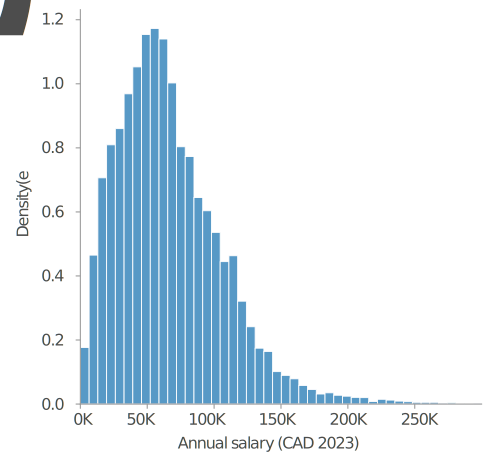
\includegraphics[width=0.58\textwidth]{images/ch4_salary_dist/salary_dist.png}
    \setlength{\abovecaptionskip}{-6pt}
    \caption{Salary distribution for the SLID dataset}
    \label{fig:salary_distribution}
\end{figure}


The comparison between average salaries by industry and the average salary in Ontario is shown in \Cref{fig:real_salary_industry}, in which both did not have significant changes during the SLID period. Some exceptions to this behaviour are the Public Administration and Utilities industries, which had an increase of 32\% and 30\% in real terms, respectively.

\begin{figure}[H]
    \centering
    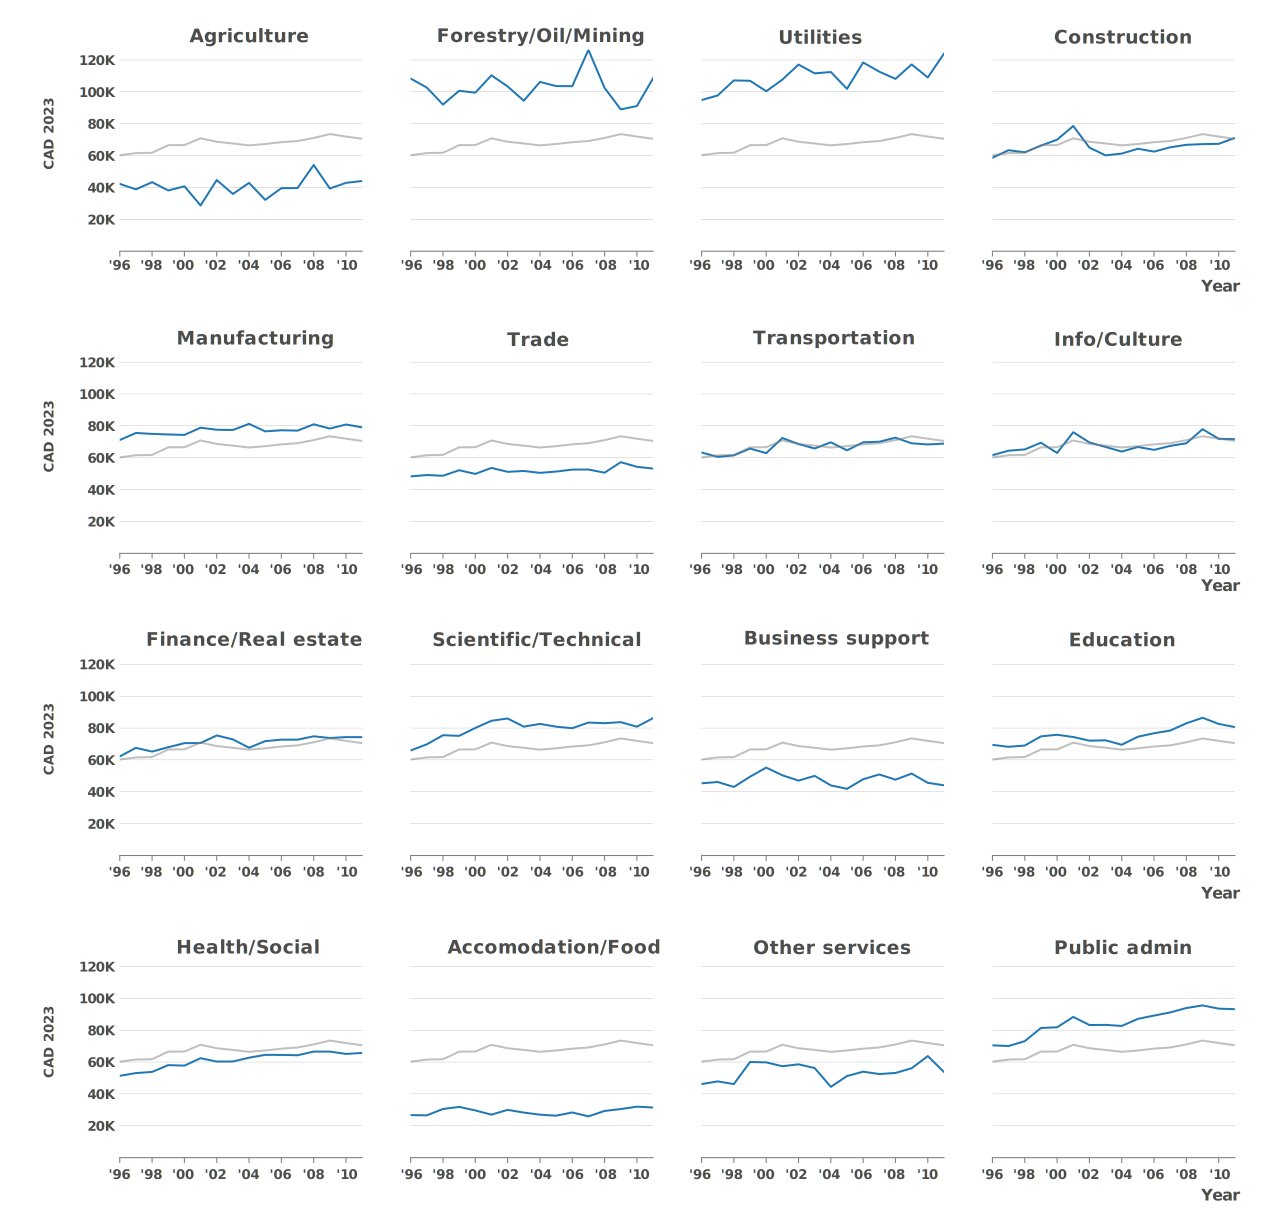
\includegraphics[width=0.97\textwidth]{images/ch4_avg_salary/avg_salary.png}
    \setlength{\abovecaptionskip}{-15pt}
    \caption{Average salary by industry in real terms (2023 Canadian dollars)}
    \label{fig:real_salary_industry}
\end{figure}

The fact that salaries in real terms did not significantly change allows the construction of models that do not consider the autoregressive nature of time series, which simplifies the modelling process and improves the interpretability of the model. 

According to the theoretical model in the literature review chapter, education level is one of the most important predictors of a person's salary because it is a proxy measure of the skill set necessary to perform a job. \Cref{fig:salary_education} shows how salary increases as the education level increases.

\begin{figure}[H]
    \centering
    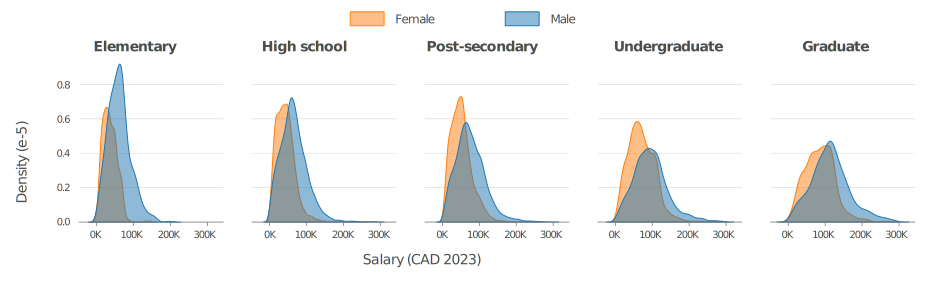
\includegraphics[width=1.0\textwidth]{images/ch4_salary_edu_gender/salary_edu_gender.png}
    \caption{Salary Distribution by education level and gender}
    \label{fig:salary_education}
\end{figure}

Although education level can explain salary increases, other variables such as age, years of experience, and tenure time at the current or previous jobs have also been associated with the salary level. As some industries and occupations require specific skills learned on the job or through many years of experience, the experience level, age or job tenure could provide more information than only using the education level. \Cref{fig:salary_pairplot} presents the pairwise relationship between these variables (first rows) and the salary (last row). 

\begin{figure}[!h]
    \centering
    \includegraphics[width=1.0\textwidth]{images/ch4_pairplot/pairplot.png}
    \setlength{\abovecaptionskip}{-10pt}
    \caption{Salaries by experience level, age, and tenure}
    \label{fig:salary_pairplot}
\end{figure}

As expected, age, experience, and tenure seem to be positively correlated. However, \Cref{fig:salary_pairplot} shows a weak linear relationship between the variables of interest and salaries, with a high variance across all data points. This variability can be explained by the hierarchical structure of the data, in which salaries are also determined by the industry and occupation. When data is filtered by industry and occupation, the linear relationship between experience, age, tenure, and salary becomes more explicit, as shown in \Cref{fig:salary_ind}. The following chapter will analyze this hierarchy in more depth to propose a model that captures this structure in the data.

\begin{figure}[!h]
    \centering
    \includegraphics[width=1.0\textwidth]{images/ch4_salary_ind/salary_ind.png}
    \setlength{\abovecaptionskip}{-10pt}
    \caption{Salary distribution by several attributes in the Public Administration industry }
    \label{fig:salary_ind}
\end{figure}

In addition to the variables supported by the theoretical models, some individual characteristics such as union participation, job sector (public or private), and employment type (self-employee or employee) were compared to assess their effect on salaries, as shown in \Cref{fig:other_fields}. Previous studies have found evidence that the effect of bargaining increases salaries because unions have more negotiating power \citep{Gregg1986,Mcdonald1992}. This negotiating power increases in some monopolistic sectors, such as the public sector, because of the lack of competition \citep{Gunderson1979}. In contrast, self-employees lack employee benefits and stability, which is directly related to lower salaries \citep{Hamilton2000}.

\begin{figure}[!h]
    \centering
    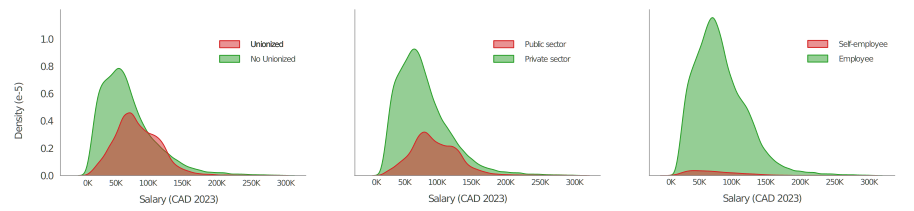
\includegraphics[width=1.0\textwidth]{images/ch4_other_fields/other_fields.png}
    \setlength{\abovecaptionskip}{-10pt}
    \caption{Salary distribution comparison between union, sector, and employment type. }
    \label{fig:other_fields}
\end{figure}